% !TeX root = ./main.tex
\documentclass[12pt,MSc,twoside]{muthesis}

\usepackage{import}
\usepackage{amsmath,amssymb}
\usepackage{graphicx}
\usepackage{tikz}
\usepackage{subfig}
\usepackage{pgfplots}
\usepackage{pgfplotstable}
\usepackage{listings}

\pgfplotsset{compat=1.5.1}

\usetikzlibrary{arrows,decorations.markings}
\tikzstyle{arrow} = [thick,->,>=stealth]

\def \oomph {\texttt{oomph-lib} }

% Define the differential d notation
\def \d{\mathrm{d}}

% Required for loading data into tables
\usepackage{csvsimple}
\usepackage{longtable}
\usepackage{array}
\usepackage{multirow}
\newcolumntype{L}[1]{>{\raggedright\let\newline\\\arraybackslash\hspace{0pt}}m{#1}}
\newcolumntype{C}[1]{>{\centering\let\newline\\\arraybackslash\hspace{0pt}}m{#1}}
\newcolumntype{R}[1]{>{\raggedleft\let\newline\\\arraybackslash\hspace{0pt}}m{#1}}

% Code style
\definecolor{dkgreen}{rgb}{0,0.6,0}
\definecolor{gray}{rgb}{0.5,0.5,0.5}
\definecolor{mauve}{rgb}{0.58,0,0.82}
\lstset{language=C++}
\lstset{frame=bt,
  language=C++,
  showstringspaces=false,
  columns=flexible,
  basicstyle={\small\ttfamily\linespread{0.7}},
  numbers=left,
  numberstyle=\tiny\color{gray},
  keywordstyle=\color{blue},
  commentstyle=\color{dkgreen},
  stringstyle=\color{mauve},
  breaklines=true,
  breakatwhitespace=false,
  tabsize=4,
  captionpos=b,
  keepspaces=true,
  showspaces=false,
  showtabs=false
}


\ifdefined\only
	\includeonly{fem}
\fi

\begin{document}

\ifdefined\nopreamble
\else
	\title{The Full Thesis Title should appear here}
\author{William Weir}
% Faculty of Life Sciences people should comment the next line out
\school{Mathematics}
\faculty{Engineering and Physical Sciences}
\def\wordcount{xxxxx}

% Uncomment the line below to suppress the `List of Tables' page (optional)
\tablespagefalse

% Uncomment the line below to suppress the `List of Figures' page (optional)
%\figurespagefalse

% Uncomment the line below to use a customised Declaration statement
%\def\declaration{All the work in this thesis has been sourced from Google.}

\beforeabstract

% Abstract

The solution to the Helmholtz equation is... 

Multigrid is an optimal solver for 

This work extends existing...

\afterabstract

\prefacesection{Acknowledgements}

I would like to thank my supervisor, Matthias Heil.
The help and support that I have received has been invaluable during this project.

Also his PhD students, Puneet Matharu and Jonathan Deakin.
Thank you for taking the time to talk through the many problems that I came up against.

Finally, I am grateful for all of the interesting discussions and biscuits at the Monday afternoon \texttt{oomph-lib} lunches.
These have introduced me to a wide range of topics that I would otherwise have not had access to.

 
\fi

\chapter{Introduction}

% Applications and who cares
The fundamental nature of waves means that waves appear in many different contexts in science, engineering, and industry.
For example, in electromagnetics, Maxwell's equations describe the physical properties of waves generated from electric and magnetic fields.
In acoustics, the propagation of sound waves may be modelled by the same equations.
Modelling of seismic waves can aid in the search for materials or objects underground and help to better understand earthquakes.
Understanding and modelling the scattering of waves is of great importance and practical use.
The equation describing the behaviour of waves in all of these applications is the wave equation, given by
\begin{align}
	\nabla^2 u = \frac{1}{c^2}\frac{\partial^2 u}{\partial t^2}, \label{eqn:first}
\end{align}
with wave speed $c$.
This is a time-dependent, second order, hyperbolic partial differential equation.
% the wave equation has widespread application and appears in
% The specific physics equation
The governing equation and the problem of interest in this project is the Helmholtz equation.
\begin{align}
	\nabla^2 u + k^2 u = 0.
\end{align}
The Helmholtz equation is a second order, elliptic type partial differential equation that arises when seeking separable solutions of the wave equation.
The physical interpretation of the solution $u$ depends on the particular application, but in general represents the amplitude of the wave with wavenumber $k$.
For our application, $u$ represents the acoustic pressure at a point in the domain.

Determining properties of an object located in a fluid is a problem applicable to many industries and fields.
For example, (Thales, defence apps)

% MAYBE CHANGE THIS, NON INFINITE CYLINDER
Consider a cylindrical object located within an infinite fluid.
We can represent the whole domain using cylindrical coordinates $(r, \phi, z)$, where $0\leq r < \infty$, $0 \leq \phi < 2\pi$, and $-\infty < z < \infty$.
If the centre of the object is located at the origin with some , then the domain contains a cylindrical hole at the origin.
Assuming symmetry of the domain about the vertical axis
By decomposing the solution into Fourier components in the azimuthal direction, we reduce the full cylindrical domain into 


% Boundary conditions
We must also specify boundary conditions for the surface of the object, as well as any other boundaries in the domain.
For an elliptic problem, all boundary edges must be specified with either Dirichlet, Neumann, or Robin conditions.
A Dirichlet condition, where the known value of the solution is given on the boundary, $u|_{\partial\Omega}=u_0$.
This type of boundary is known as soft, and can be interpreted as the boundary of an elastic wall that is displaced in response to a force on the outside.
A value of zero on the boundary is known as a pressure release boundary.
If the value here is nonzero, the boundary experiences some force from the other side.
For a Neumann boundary, the normal derivative $\vec{n}\cdot \nabla u |_{\partial \Omega} = \partial u / \partial \vec{n} |_{\partial \Omega}$ is given on the boundary.
The physical interpretation of this is a hard boundary, that does not move in response to a force.
Lastly a Robin condition, giving both the value of the solution and the normal derivative on the boundary can be interpreted as a combination of the two above.



% Sommerfeld + truncation
In addition to boundary conditions, an additional condition on the solution must be imposed to ensure that the solution is unique since the domain of the problem is infinite.
The Sommerfeld radiation condition in three dimensions is given by
\begin{align}
	\lim_{|x|\rightarrow \infty} |x| \left( \frac{\partial}{\partial |x|} - ik \right) u(x) = 0. \label{eqn:sommerfeld}
\end{align}
This achieves this requirement by ensuring that sources scatter to infinity and do not come from infinity \cite{sommerfeld}.

Because the problem is defined on an infinite domain, we must perform a truncation of the domain to find the solution numerically.
Choosing some appropriately sized region of interest surrounding the object, we restrict the domain to this region.
However, this causes problems with waves interacting with the boundary of the truncated domain.
Spurious waves from reflections on the outer walls propagate through the domain and the resulting solution is no longer correct.
It is possible to deal with these reflections by introducing an artifical absorbing layer to the boundary of the domain.
Several such layers exist, for instane absorbing boundary conditions (ABCs); Dirichlet-to-Neumann condtions (DtNs); and perfectly matched layers (PMLs).
These all attempt to dampen waves in the artificial layer surrounding the domain so that there are no reflections back into the domain.



% ----------------------------------------------

% How do we solve the problem
\iffalse
	Discretise
	Direct vs Iterative solver (Krylov subspace)
	Multigrid
	Preconditioners
	CSLP
	MG as a preconditioner
\fi

% FEM Discretisation
In order to solve the problem, we will use the C++ library \oomph to find the solution using the finite element method.
This process will involve the discretisation of the equations on each element of the domain with the resulting system being assembled.
The result of the finite element discretisation is an $n\times n$ linear system of equations,
\[
	A x = b,
\]
which requires a solver in order to compute the solution.
In \oomph, the default linear solver is SuperLU, however this is also a direct solver.
This has the benefit that the computed solution to the above equation is exact, modulo any floating point errors.
But the computational cost is prohibitively expensive as the size of the problem increases.

% Direct vs Iterative methods
For small $A$, it is possible to use direct methods to solve these exactly (in exact arithmetic).
As is often the case in practice, the matrices from the finite element discretisation are too large to compute by direct methods.
Instead, many iterative methods have been developed to approximate the solution instead.
A particular class of methods, Krylov subspace methods, form the solution by building iterates from elements in a space  of successive powers of the matrix $A$ \cite{leveque}.
The Krylov space of dimension $k$ is 
\[
	\mathcal{K}_k(A, r_0) = \mathrm{span}(r_0, Ar_0, A^2 r_0, \ldots, A^{k-1} r_0).
\]
Such methods include the conjugate gradient and GMRES methods.

% Preconditioning
This equation is generated from the finite element discretisation of the problem.
Linear systems of equations are everywhere, so there are a choice of several different methods to use to solve.
Direct methods are too costly to use since in general, the dimension of the problem is large.
Iterative methods, such as Krylov subspace methods, are a good alternative to use.
However the performance of such methods is poor without a preconditioner.
Hence, we would like a preconditioner that improves the performance of the iterative method.

Applying a preconditioning matrix $P$ on the left, we have
\begin{align}
	P^{-1} A x = P^{-1} b, \label{eqn:precond_left}
\end{align}
which solves the above system exactly for the case $P=A^{-1}$. 
This is optimal as it solves the original problem, however it is costly to obtain.
Instead, we would like a alternative such that $P$ is cheap to find and the preconditioned system \eqref{eqn:precond_left} is easier to solve than the original problem.

Alternatively, a preconditioning matrix can be applied on the right.
In this case, we have
\begin{align}
	A P^{-1} P x = b. \label{eqn:precond_right}
\end{align}
This can be solved in two steps, 
\begin{align}
	P x = y, \\A P^{-1} y = b.
\end{align}


Many general preconditioning techniques have been developed that work for a wide variety of problems.
For example, preconditioning matrices based on the splitting of the matrix $A$ are simple to use and cheap to compute.
More specific preconditioning techniques have been developed in the case of certain problems.
These tend to be more complicated to use, but often will come with better performance.
As a first attempt, it is a good idea to use a simple method to see the impact on the convergence times.
Only in the case where optimisation is crucial to the problem or a general preconditioner does not work, a specific preconditioner should be developed.


% Multigrid
% Need more at the beignning
% MULTIGRID http://www.mgnet.org/mgnet/books/Wesseling/bookr-orig.pdf
Wesseling describes the historical development of multigrid methods from their inception in 1967 up to 1985 \cite{wesseling}.
It is stated that the first mention of multigrid was by the Russian mathematician Fedorenko.
In his paper, Fedorenko developed a method for solving elliptic type partial differential equations, which he called the ``the method of alternating direction'' \cite{fedorenko}.
Later, Hackbusch independently developed multigrid methods and presented the rigorous mathematical framework for multigrid.

Since multigrid was developed in order to find solutions to elliptic problems, the majority of work has been focused in that area.
As the prototypical example of an elliptic PDE is Poisson's equation, we can be certain that the mathematical framework for solving this is set.
The difficulty lies with the Helmholtz equation, which can be thought of a perturbation by $k^2$ of the Laplace operator in the Poisson equation.
As both the Poisson and Helmholtz equations are both of elliptic type, we should expect behaviour to be similar.
However, this is not the case.

The performance of multigrid methods is excellent for the related Poisson problem,
\begin{equation}
	\nabla^2 u = f. \label{eqn:poisson}
\end{equation}
Indeed, it is an optimal solver with time-complexity of $O(n)$ for a problem of size $n\times n$.
For sufficiently small values of $k$, the Helmholtz equation is well approximated by Poisson's equation.
In addition, the matrix arising from the finite element discretisation is well-conditioned.
As $k$ becomes larger, however, the matrix becomes indefinite and more and more ill-conditioned.
This causes multigrid to fail to converge to a solution.
To handle the ill-conditioned system, a preconditioner can be used so that the problem may be more easily solved by numerical methods.

The multigrid solver for the Helmholtz equation exists for the equation in Cartesian coordinates in \oomph.
We would like to explore the performance of the solver for the Fourier decomposed version of the Helmholtz equation in axisymmetric cylindrical coordinates.
Following this, we will also examine the performance of the solver using PMLs to handle reflections on the discretised boundary.


% Multigrid as a preconditioner
Multigrid methods may also be used as a preconditioner for other iterative methods.
With a reduced

Since at each iteration of the outer iterative method the preconditioner will change, the iterative method must be `flexible'.
Saad created the Flexible GMRES iterative method, FGMRES \cite{fgmres}.
This is the solver used to solve the linear system 


% CSLP
Work on overcoming the issue for larger values of $k^2$ has been successful.
The current preferred method for solving the problem is to precondition a Krylov subspace method using a complex-shifted laplacian preconditioner (CSLP).
Convergence results obtained by authors Erlangga, Oosterlee, and Vuik show that among the class of preconditioners discussed, the CSLP is the most effective in preconditioning the Helmholtz problem for large wavenumber \cite{cslp1}.
They showed... % DISCUSSION OF THE FIRST PAPER

In a second paper by the same authors, they go on to discuss the CSLP in more detail, and in particular, applied to multigrid methods \cite{cslp2}.
% DISCUSSION OF THE SECOND PAPER









% -----------------------------------------------

\section{Project outline}

Chapter one contains the introduction to the project.
This has hopefully given you, the reader, the modern and historical context of the problem of interest, as well as the aims and objectives to motivate the rest of this dissertation.

The focus of chapter two is to derive the mathematics of the problem.
Here we will give the necessary mathematical overview and description of the problem and the derivation of equations.
Also here will be issues associated with the practicalities of finding a solution.

Chapter three aims to cover the necessary high level facets of the finite element method for the the problem in question.
Also covered are relevant references to the FEM implementation within \oomph and how the mathematical description of the FEM is transferred to an object-oriented code able to solve PDEs numerically.

Chapter four will motivate multigrid and outline the mathematics of the multigrid algorithm for solving the Helmholtz equation.
In particular, we discuss the application of multigrid in finding the solution to the finite element discretisation of the Helmholtz equation.

The project will come together at the end with a discussion of the results.
Here, a summary of findings and an overview of the work completed in the project will be given, as well as comparison to related problems and the current literature.

Finally, we will complete the dissertation with concluding remarks and outline steps for moving forward from the end of the project.
\chapter{The problem}
\label{sec:problem}

\iffalse

Background definitions, notations, etc.
Problem definition
	- Relation to Helmholtz
Boundary condition
	- Sommerfeld
	- PML/ABC/DtN
Shifted Laplace operator


The Poisson problem:
	- Well behaved
	- Eigenvalues of the residual
	- Optimal method for finding solution

Helmholtz problem:
	- Misbehaved
	- Poor convergence
	- Indefinite discretisation matrix
\fi

The end goal is to solve the Helmholtz equation in cylindrical coordinates in an unbounded three-dimensional domain, with symmetry about the $z$-axis.
Simplifying slightly, we assume a finite domain with Dirichlet boundary conditions on the exterior walls.
We also assume that the object has vertical length equal to the height of the domain, also with Dirichlet boundary conditions.
This is justified since we are not interested in the solution to the problem, rather than the behaviour of the method in finding the solution.

In this chapter, we will derive the formal statement of the problem starting from the wave equation.
Also included here is a discussion of the topics relevant to the practical solution of the problem.
The final outcome of this chapter should be the starting point for the finite element discretisation in chapter \ref{sec:fem}.




% ------------------------------

\section{Problem derivation}

Consider the three dimensional wave equation with wave speed $c$,
\begin{equation}
	\frac{1}{c^2} \frac{\partial^2 u(x,y,z,t)}{\partial t^2} = \nabla^2 u(x,y,z,t). \label{eqn:wave}
\end{equation}
Following \cite{oomph_hh}, we assume the existence of a separable solution where the time component of the solution is time-harmonic with frequency $\omega$.
We may write the real-valued solution as
\[
	u(x,y,z,t) = \Re \left( U(x,y,z)e^{-i\omega t} \right),
\]
where $U(x,y,z)$ is a complex-valued function.
Substituting this into \eqref{eqn:wave}, we obtain the Helmholtz equation
\begin{equation}
	\nabla^2 U(x,y,z) + k^2 U(x,y,z) = 0, \label{eqn:hh}
\end{equation}
where the wavenumber $k$ is defined as
\begin{align}
	k = \frac{\omega}{c}.
\end{align}

The mapping between Cartesian coordinates $(x,y,z)$ and cylindrical polar coordinates $(r,\varphi,z)$ is given by
\begin{align}
	x &= r\cos(\varphi), \\
	y &= r\sin(\varphi), \\
	z &= z.
\end{align}
The Jacobian of this mapping is given by
\begin{align}
	J = \left\vert \frac{\partial(x,y,z)}{\partial(r,\varphi,z)} \right\vert = r. \label{eqn:cylindrical_mapping}
\end{align}
This mapping transforms our equation from $U(x,y,z)$ into $U(r,\varphi,z)$, 
which we may decompose into its Fourier components $u_N(r,z)$ around the $z$-axis, so that
\begin{equation}
	U(r,\varphi,z) = \sum_{N=-\infty}^\infty u_N(r,z) e^{iN\varphi}. \label{eqn:full_eqn}
\end{equation}
By linearity of the Helmholtz equation, for each $N$, $u_N(r,z)$ must satisfy the Helmholtz equation.
This allows us to solve for each $N$ individually and then combine the solutions to form a full solution.

The Laplacian in cylindrical coordinates is given by
\begin{align}
	\nabla^2 = \frac{\partial^2 }{\partial r^2}
			 + \frac{1}{r} \frac{\partial }{\partial r}
			 + \frac{1}{r^2} \frac{\partial^2 }{\partial \varphi^2}
			 + \frac{\partial^2 }{\partial z^2}. \label{eqn:laplacian}
\end{align}
We also define the reduced Laplacian in cylindrical coordinates, consisting of only partial derivatives with respect to $r$ and $z$.
\begin{align}
	\nabla^2 = \frac{\partial^2 }{\partial r^2}
			 + \frac{1}{r} \frac{\partial }{\partial r}
			 + \frac{\partial^2 }{\partial z^2}. \label{eqn:laplacian_reduced}
\end{align}
It is not necessary to distinguish between the two operators \eqref{eqn:laplacian} and \eqref{eqn:laplacian_reduced}.
In the case of a function in $(r,\varphi,z)$, then the full cylindrical Laplacian is required.
Alternatively, for a function in $(r,z)$, the reduced cylindrical Laplacian is appropriate.
Therefore the distinction should be implicit from the context of the equation.

Hence above, we wish to extract those terms consisting of $\varphi$ from \eqref{eqn:full_eqn}.
The partial derivatives with respect to $\varphi$ give
\begin{align}
	\frac{1}{r^2} \frac{\partial^2 }{\partial \varphi^2} \left( e^{i N \varphi}\right) = - \frac{N^2}{r^2} e^{i N \varphi}.
\end{align}
The Laplacian term of the equation is
\begin{align}
	\nabla^2 U(r,\varphi,z) 
		&= \nabla^2 \left[\sum_{N=-\infty}^\infty u_N(r,z) e^{i N \varphi}\right] \\
		&= \sum_{N=-\infty}^\infty \left[ 
										\nabla^2 u_N(r,z) - \frac{N^2}{r^2}u_N(r,z)
								   \right] e^{i N \varphi}.
\end{align}
We can then add on the $k^2$ term to find the full equation.

Since we can solve each term in the series separately, we can extract a single equation for each $N$.
This gives us the Fourier decomposed Helmholtz equation,
\begin{equation}
	\nabla^2 u_N(r,z) + (k^2 - \frac{N^2}{r^2})u_N(r,z) = 0. \label{eqn:fhh}
\end{equation}

The standard Helmholtz equation is classified by a single parameter, the wavenumber $k$.
Decomposing the solution into Fourier components, we introduce the Fourier wavenumber $N$ as an additional parameter to the system.
These two parameters together determine the equation and thus the solutions for the problem.







% ----------------------------------------

\subsection{Multigrid for the Helmholtz equation}

There are difficulties in solving the Helmholtz equation using multigrid as the solver.
This is especially true for even moderate values of $k^2$.
Large values of $k^2$ cause the discretisation matrix to be indefinite, causing the solver to not converge.
Work has been done by several authors in order to overcome this shortcoming of multigrid \cite{cslp1, cslp2}.

Multigrid performs poorly for the Helmholtz equation due to the indefiniteness of the operator.
However, multigrid is a good solver for the nearby problem shifted into the complex plane.
This is not the problem we want to solve, but a good enough approximation to use as a preconditioner for another iterative method.

Introducing a shift to the complex plane, the Helmholtz operator in Cartesian coordinates becomes
\begin{align}
	\mathcal{L}_{CSLP} = \nabla^2 + (1 + i \alpha ) k^2,  \label{eqn:cslp}
\end{align}
where $\alpha$ is a positive real number controlling the offset from the real axis.

Since our equation is defined in Fourier decomposed cylindrical coordinates, we obtain for the Fourier decomposed Helmholtz equation,
\begin{align}
	\nabla^2 u_N(r,z) + \left[ \left( 1 + i \alpha \right) k^2 - \frac{N^2}{r^2} \right] u_N(r,z) = 0.
\end{align}
Here, the shift is still applied to the $k^2$ term, but we have the additional term from \eqref{eqn:fhh}.

The optimal value of $\alpha$ is determined in \cite{cslp2}.
Specifically, they state that taking $\alpha=0.5$ yields the best possible results.
In all of our numerical experiments, we will use this value for the multigrid preconditioner.








% ----------------------------------------

\section{Related problems and other issues}

In the case where $k^2=0$, the problem reduces to the Poisson problem \eqref{eqn:poisson} with $f=0$, otherwise known as Laplace's equation.
Taking $k^2=0$ in equation \eqref{eqn:fhh}, we obtain
\begin{align}
	\nabla^2 U(r,\varphi,z) = \nabla^2 u_N(r,z) - \frac{N^2}{r^2} u_N(r,z) = 0. \label{eqn:fp}
\end{align}
This is Poisson's equation in Fourier decomposed cylindrical coordinates.

The Poisson equation is of interest because of the close relation between the Helmholtz and Poisson equations.
It is known that multigrid performs optimally for Poisson's equation.
Since we are interested in how multigrid performs when solving \eqref{eqn:fhh}, we will compare results with this equation.

Another related problem is the case when both $k^2=0$ and $N=0$.
This is the Poisson equation in reduced axisymmetric coordinates, where the solution depends only on $r$ and $z$.
To further aid in comparison between solutions, we will also consider how the equation behaves in this case.


% Variable coefficients --------------

A common issue arising when using a multigrid solver occurs with variable coefficient problems \cite{briggs}.
In Cartesian coordinates, the Helmholtz equation is a constant coefficient problem.
This is seen in the operator
\begin{align}
	\nabla^2 + k^2 = \frac{\partial^2}{\partial x^2} + \frac{\partial^2}{\partial t^2} + \frac{\partial^2}{\partial z^2} + k^2.
\end{align}

In cylindrical coordinates, however, we have a terms that vary proportionally to the inverse of the radial distance and the radial distance squared.
For the Fourier decomposed Helmholtz equation, recall equation \eqref{eqn:fhh},
\begin{align}
	\frac{\partial^2 u_N}{\partial r^2}
			 + \frac{1}{r} \frac{\partial u_N}{\partial r}
			 + \frac{\partial^2 u_N}{\partial z^2}
			 + (k^2 - \frac{N^2}{r^2})u_N = 0. \label{eqn:full_fhh}
\end{align}
As suggested in the literature, this may cause issues with multigrid.
A test of the method should be performed first to confirm before attempting to remedy potentially non-existent issues with variable coefficients.









% ----------------------------------------

\section{Domain and boundary conditions}

The full wave equation \eqref{eqn:wave} is defined in three spatial dimensions and one temporal dimension.
The full cylindrical Helmholtz equation \eqref{eqn:full_eqn} is defined in a cylinder in three spatial dimensions.
If we let the cylindrical domain have a maximum radius of $R_{\mathrm{max}} > 0$, and let the domain contain a cylindrical cavity with some maximum radius $0<R_{\mathrm{min}}<R_\mathrm{max}$.
The resulting domain is shown in figure \ref{fig:full_domain}.

In the reduced $(r,z)$ coordinates for the Fourier decomposed equation \eqref{eqn:fhh}, the domain becomes \ref{fig:reduced_domain}.
This simplification aids in the computational work by reducing the number of degrees of freedom of the problem.
It is only a matter of post-processing the solution to obtain the full 3D solution from the reduced computed solution, as nothing is lost due to symmetry.
To obtain the full domain from this, a rotation of $2\pi$ radians about the $z$-axis is performed.

To complete the problem formulation, boundary conditions must also be specified for the PDE.
The boundaries we need to specify on are the inner regions of the cylindrical walls.
This translates to the four boundaries in the reduced equation.
The Dirichlet boundary conditions on the entire boundary are then
\begin{align}
	u_N(r,z) = u_0 \quad \mathrm{on} \quad \partial \Omega,
\end{align}
for some given value of $u_0$.



\begin{figure}[ht!]
	% Need an example image of a 3d cylinder - the domain for the problem -- away from the 
	% Also the 2d section of the cylinder
	\centering
	\subfloat[][Full cylindrical domain. \label{fig:full_domain}]{
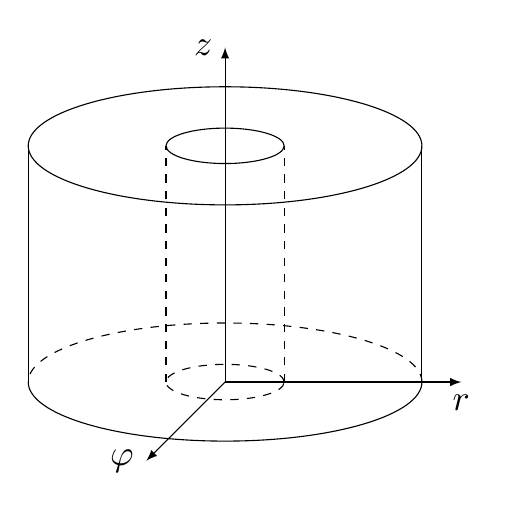
\begin{tikzpicture}[scale=2.5, >=latex]
  % AXES
  % z-axis
  \draw[->] (0.5,0) -- (0.5,1.7) node[left, scale=1.3] {$z$};
  % r-axis
  \draw[->] (0.5,0) -- (1.7,0) node[below, scale=1.3] {$r$};
  % phi-axis
  \draw[->] (0.5,0) -- (0.1,-0.4) node[left, scale=1.3] {$\varphi$};

  % INNER CYLINDER
  % top ellipse
  \draw[solid] (0.5,1.2) ellipse (0.3 and 0.09);
  % bottom ellipse
  \draw[dashed] (0.5,0) ellipse (0.3 and 0.09);
  
  % left line
  \draw[dashed] (0.2,0) -- ++(0,1.2);
  % right line
  \draw[dashed] (0.8,0) -- ++(0,1.2);


  % OUTER CYLINDER
  % top ellipse
  \draw[solid] (1.5,1.2) arc (0:180:1 and 0.3);
  \draw[solid] (-0.5,1.2) arc (180:360:1 and 0.3);
  % bottom ellipse
  \draw[dashed] (1.5,0) arc (0:180:1 and 0.3);
  \draw[solid] (-0.5,0) arc (180:360:1 and 0.3);
  
  % left line
  \draw (-0.5,0) -- ++(0,1.2);
  % right line
  \draw (1.5,0) -- ++(0,1.2);
\end{tikzpicture}	
	}\quad
	\subfloat[][Reduced dimensional domain. \label{fig:reduced_domain}]{
		\begin{tikzpicture}[scale=3, >=latex]
  % z-axis
  \draw[->] (0,0) -- ++(0,1.6) node[left, scale=1.3] {$z$};
  % r-axis
  \draw[->] (0,0) -- ++(1.7,0) node[below, scale=1.3] {$r$};

  \draw[solid] (0.3,0.15) -- ++(1,0) -- ++(0,1.2) -- ++(-1,0);
  \draw[dashed] (0.3,0.15) -- ++(0,1.2);

\end{tikzpicture}
	}
	\caption{Problem domain.\label{fig:problem_domain}}
\end{figure}









% --------------------------------------

\section{An analytical solution}

In order to show that the computed solution of a numerical method is producing accurate results, a known solution is required to validate results.
The 3D axisymmetric domain reduces to a 2D rectangle that sweeps around the $z$-axis.
Hence, we want to find an analytical solution on a rectangle in $r$ and $z$ coordinates.

Let us begin by assuming the existence of a separable solution,
\begin{align}
	u_N(r,z) = R(r)Z(z).
\end{align}
Substituting into \eqref{eqn:fhh}, we obtain
\begin{align}
	\left( \frac{\d^2 R(r)}{\d r^2} + \frac{1}{r} \frac{\d R(r)}{\d r} \right) Z(z) + \frac{\d^2 Z(z)}{\d z^2} R(r) + \left( k^2 - \frac{N^2}{r^2} \right) R(r) Z(z) = 0.
\end{align}
Dividing through by $R(r)Z(z)$, we can separate terms consisting of $r$ and $z$ on each side of the equation.
\begin{align}
	\left( \frac{\d^2 R(r)}{\d r^2} + \frac{1}{r} \frac{\d R(r)}{\d r} \right)\frac{1}{R(r)} + \left( k^2 - \frac{N^2}{r^2} \right) = - \frac{\d^2 Z(z)}{\d z^2} \frac{1}{Z(z)}.
\end{align}
Because both sides of this equation are equal expressions involving different variables, they must be equal to some constant, say $\lambda$, whose sign is yet to be determined.
Hence, we obtain two ordinary differential equations in $r$ and in $z$.
\begin{align}
	&\frac{\d^2 Z(z)}{\d z^2} + \lambda Z(z) = 0. \label{eqn:Z}\\
	&\frac{\d^2 R(r)}{\d r^2} + \frac{1}{r} \frac{\d R(r)}{\d r} + \left( k^2 + \lambda - \frac{N^2}{r^2} \right) R(r) = 0. \label{eqn:R}
\end{align}


First, we solve \eqref{eqn:R} for $R(r)$.
Consider the change of variables
\begin{align}
	\tilde{r} = r \sqrt{k^2 + \lambda}.
\end{align}
By the chain rule, derivatives in $\tilde{r}$ become
\begin{align}
	\frac{\d R}{\d r} &= \frac{\d \tilde{r}}{\d r} \frac{\d R}{\d \tilde{r}} = \sqrt{k^2 + \lambda} \frac{\d R}{\d \tilde{r}} \\
	\frac{\d^2 R}{\d r^2} &= \sqrt{k^2 + \lambda} \frac{\d}{\d \tilde{r}} \left[ \sqrt{k^2 + \lambda} \frac{\d R}{\d \tilde{r}} \right]
							= \left(k^2 + \lambda\right) \frac{\d^2 R}{\d \tilde{r}^2}
\end{align}
Substituting into \eqref{eqn:R}, 
\begin{align}
	\left(k^2 + \lambda\right) \frac{\d^2 R(\tilde{r})}{\d \tilde{r}^2} + 
	\frac{\left(k^2 + \lambda\right)}{\tilde{r}} \frac{\d R(\tilde{r})}{\d \tilde{r}} + 
	\left(k^2 + \lambda\right) \left( 1 - \frac{N^2}{\tilde{r}^2} \right) R(\tilde{r}) = 0.
\end{align}
Upon cancelling factors, we have the final equation, which may be recognised as Bessel's differential equation.
\begin{align}
	\frac{\d^2 R(\tilde{r})}{\d \tilde{r}^2} + 
	\frac{1}{\tilde{r}} \frac{\d R(\tilde{r})}{\d \tilde{r}} + 
	\left( 1 - \frac{N^2}{\tilde{r}^2} \right) R(\tilde{r}) = 0. \label{eqn:bessel_de}
\end{align}
The solution to \eqref{eqn:bessel_de} is a linear combination of Bessel functions of order $N$, and whose argument is $\tilde{r}=r \sqrt{k^2 + \lambda}$.
\begin{align}
	R(r) = c_1 J_N \left( r \sqrt{k^2 + \lambda} \right) + c_2 Y_N \left( r \sqrt{k^2 + \lambda} \right)
\end{align}


Now we turn to the solution of \eqref{eqn:Z}.
The form of the solution of $Z(z)$ is depending on the sign of $\lambda$.
Let $\mu$ be a positive real number.
If the sign is negative so that $\lambda=-\mu^2$, then $Z(z)$ is a linear combination of hyperbolic sine and cosine,
\begin{align}
	Z(z) = c_3 \sinh(\mu z) + c_4 \cosh(\mu z).
\end{align}
On the other hand, if the sign is positive, so that $\lambda=\mu^2$, then $Z(z)$ is a linear combination of sine and cosine,
\begin{align}
	Z(z) = c_3 \sin(\mu z) + c_4 \cos(\mu z).
\end{align}
Finally, if $\lambda=0$, then $Z(z)$ is the equation of a straight line,
\begin{align}
	Z(z) = c_3 z + c_4.
\end{align}

For the sake of simplicity, we can specify that $\lambda=0$.
We have then for the full general solution for a single Fourier mode,
\begin{align}
	u_N(r,z) = R(r)Z(z) = \left( c_1 J_N \left( k r \right) + c_2 Y_N \left( k r \right) \right) \left( c_3 z + c_4 \right),
\end{align}
for any given constants $c_1,c_2,c_4,c_4$.

Since the only purpose of this exact solution is for validation of a correct implementation, we may choose the constants above freely.
In doing so, we may then specify that the boundary conditions for the PDE must correspond with the exact solution.
That is, since we know a priori the solution of the equation, we let the boundary conditions be exactly the value of the solution on the boundary.
This has the benefit of finding the solution we have found above for us to check the method against.
Although this has the distinct disadvantage that we do not make use of any boundary conditions besides Dirichlet conditions.

\chapter{The finite element method}
\label{sec:fem}

This chapter discusses the well known and widely used method for solving partial differential equations, the finite element method (FEM).
To avoid building and adding another library to the already vast ecosystem of available FEM software, we use the multi-physics FEM library, \oomph.
From the website, \oomph is:
\begin{quote}
	an object-oriented, open-source finite-element library for the simulation of multi-physics problems. \cite{oomph}
\end{quote}
There are several high level features of any general finite element procedure that will be addressed below.
Discussing these features in generality allows for specificity later to any problem.
However, we will also be explicit with description about the problem referenced earlier.
In addition to this, an overview of specific implementation details and features available in \oomph will also be covered.





% -----------------------------------------------------------

\section{Preliminaries}

\iffalse

.Problem
.Classical vs weak solution
Test functions
Sobolev space (where test functions live)
Basis/shape functions
Galerkin method -> test functions are basis functions

\fi

We begin this chapter by discussing the necessary mathematical background for the finite element method.

The classical or strong solution of a problem is a function $u_N(r,z)$ satisfying the PDE
\begin{align}
	\nabla^2 u_N + \left[ (1+i\alpha)k^2-\frac{N^2}{r^2}\right]u_N = 0,
\end{align}
at every point in the domain $\Omega$ and satisfying the boundary conditions
\begin{align}
	u_N(r,z) \vert_{\partial \Omega_D} = g_D \\
	\frac{\partial u_N(r,z)}{\partial \vec{n}} \vert_{\partial \Omega_N} = g_N
\end{align}
at every point on the respective portion of the boundary $\partial\Omega$.

The weak solution of a problem is a relaxation of the conditions for the existence of a solution to the problem.
A weak solution $u_N^{\mathrm{weak}}(r,z)$ satisfies the essential (Dirichlet) boundary condition and that
\begin{align}
	\int_\Omega \left( \nabla^2 u_N + \left[ (1+i\alpha)k^2-\frac{N^2}{r^2}\right]u_N \right) v = 0
\end{align}
for all test functions $v$ that are 0 on the essential boundary.

The test functions are used to weight the integral of the residual equation and are members of the function space
\begin{align}
	H^1_0(\Omega) = \left\{ v | v=0 \mathrm{on} \partial\Omega_D, \, v \in L^2(\Omega), \, \nabla v \in (L^2(\Omega))^2 \right\}.
\end{align}
The solution $u_N^{\mathrm{weak}}(r,z)$ must satisfy the Dirichlet boundary condition, and so is a member of the space
\begin{align}
	H^1(\Omega) = \left\{ v | v \in L^2(\Omega), \, \nabla v \in (L^2(\Omega))^2 \right\}
\end{align}
The function spaces $H^i(\Omega)$ are known as Sobolev spaces and are complete normed vector spaces.


% For the strong form above, we require at least that $u_N(r,z) \in C^2(\Omega)$.
% A sufficiently smooth solution satisfying the weak form will also satisfies the stong form.
% Therefore the two statements of the problem are equivalent, given the smoothness requirements of the classical formulation.


The solution on the mesh is represented using shape functions that form a basis for the domain.

For a two-dimensional domain, the shape functions are bilinear and 
In particular, for the global node $j$ in the mesh, the basis function $\phi_j(r,z)$ is 1 at node $j$ and 0 everywhere else.


Local vs global coordinates




% -----------------------------------------------------------

\section{Nodes, elements, and meshes}

The main components of the finite element method are the nodes, the elements, and the mesh.
A mesh is a collection of elements; an element is a collection of nodes.

Each node contains data about its location within the mesh, its local coordinate within the element, as well as the value of the solution at the node.

The elements are the 

The number of nodes of an element determines its order.
If For example, an element with

How do we get from global to local coordinates?
We need the mapping
And with that we need the Jacobian of the mapping
(we have two change of coordinates: Cartesian -> Cylindrical -> Local
And so we have two Jacobian mappings)

On the elements we have defined basis functions.
These represent the function 

Together with the elements, other fundamental pieces of the FEM are the nodes and the mesh.
Every element consists of multiple nodal points, each of which holds data required for solving the problem.
For example, nodes contain the global coordinate of their position within the mesh



The FEM lends itself well to object-oriented programming (OOP) design principles.
This is due to the discrete entities involved and the relationships between them.
Such a design strategy involves the definition of classes, and their instantiation as objects.
Furthermore, classes may be extended using inheritance, allowing for highly abstracted and generic classes, and on the other end, highly specific classes.
This is an advantage for both the developers and the users of \oomph.
Developers are able to work independently of each other, knowing only how objects should interact.
Users are able to extend previous work to suit their own needs.






% -----------------------------------------------------------

\section{Weak formulation}

We will now derive the weak form of the CSLP equation, \eqref{eqn:cslp}.
Our first step is to multiply the equation by a test function $v\in H^1_0(\Omega)$ and integrate over the domain $\Omega$.
\begin{align}
	-\int_\Omega \left(\nabla^2 u_N + \left[ (1+i\alpha)k^2-\frac{N^2}{r^2}\right]u_N \right) v = 0.
\end{align}
Using the property of the gradient operator,
\begin{align}
	\nabla \cdot ( v \nabla u) = v \nabla^2 u + \nabla u \cdot \nabla v,
\end{align}
we arrive at
\begin{align}
	\int_\Omega \nabla u_N \cdot \nabla v 
  - \int_\Omega \nabla \cdot (v \nabla u ) 
  - \int_\Omega \left[(1+i\alpha)k^2 - \frac{N^2}{r^2}\right] u_N v = 0.
\end{align}

Using the Gauss-Divergence theorem, we may write the second term as an integral over the boundary of the domain $\partial \Omega$,
\begin{align}
	\int_\Omega \nabla \cdot (v \nabla u ) = \int_{\partial\Omega} v \frac{\partial u_N}{\partial \vec{n}},
\end{align}
where $\vec{n}$ is the outward facing normal vector from the boundary.
The boundary integral may be further split up into parts sorted by their respective boundary conditions.
If the portion of the boundary whose solution value is known is represented by $\partial \Omega_D$ and the remaining boundary is represented as $\partial \Omega_N$, then
\begin{subequations}
\begin{align}
	\partial \Omega_D \cup \partial \Omega_N &= \partial \Omega. \\
	\partial \Omega_D \cap \partial \Omega_N &= \emptyset.
\end{align}
\end{subequations}
Given these exclusivity properties on the boundary, we may write the term for the boundary integral as
\begin{align}
	\int_{\partial\Omega} = \int_{\partial\Omega_D} + \int_{\partial\Omega_N}.
\end{align}
Since by definition, the test functions are exactly 0 on the Dirichlet portion of the boundary, it is the case that
\begin{align}
	\int_{\partial\Omega_D} v \frac{\partial u_N}{\partial \vec{n}} = 0.
\end{align}
We will also consider a boundary with only Dirichlet conditions, so that the Neumann part also vanishes.

Combining the results, we arrive at the weak form: find $u_N(r,z) \in H^1(\Omega)$ such that for all $v \in H^1_0(\Omega)$,
\begin{align}
% 	\int_\Omega \nabla u_N \cdot \nabla v 
%   - \int_{\partial\Omega_N} \nabla \cdot (v \nabla u_N ) 
%   - (1+i\alpha)k^2 \int_\Omega u_N v 
%   - N^2 \int_\Omega \frac{1}{r^2} u_N v = 0. \label{eqn:weakform}
	\int_\Omega \left[
		\nabla u_N \cdot \nabla v 
	  - \left((1+i\alpha)k^2 - \frac{N^2}{r^2}\right) u_N v 
	\right] = 0. \label{eqn:weakform}
\end{align}


One further point regarding the implementation of this within \oomph.
Complex numbers are not handled natively within \oomph.
Instead, a two-dimensional vector whose first and second components store the real and imaginary parts of a complex number, respectively.
Therefore to deal with this, we split the solution $u_N$ into its real and imaginary components.
If $u_r$ is the real part of the solution and $u_c$ is the imaginary part, then
\begin{align}
	u_N = u_r + i u_c.
\end{align}
Substituting this into \eqref{eqn:weakform} and separating real and imaginary parts will acheive this.







% ----------------------------------------------------------

\section{Numerical integration}
\label{sec:integration}

The integrals involved in computing the solution are often too complicated evaluate analytically.
Instead, we use a numerical integration scheme to perform the integration.
Several methods exist to complete this task, but within \oomph, it is done using Gauss quadrature.

\cite{oomph}
Fix the dimension to be 2, so that we can talk specifics...
The Gauss rules are defined by following three quantities:
\begin{enumerate}
	\item the number of integration points, $N_\mathrm{int}$,
	\item the position of the integration points within an element, $S_i, \, i=1,2,\ldots,N_\mathrm{int}$,
	\item the integration weights, $W_i, \, i=1,2,\ldots,N_\mathrm{int}$.
\end{enumerate} 
Given these values, we can approximate an integral by summation of the integrand evaluated at the integration points multiplied by the corresponding integration weight.

We also must multiply by the Jacobian of the mapping from Cartesian to cylindrical coordinates.
Recall equation \eqref{eqn:cylindrical_mapping}, which states that the Jacobian of this transformation is $r$.
In addition, we have the transformation from global to local coordinates.
This mapping is given by some other function

Denote by $J$ the Jacobian of the mapping from global to local coordinates, then for an arbitrary element $E$, 
\begin{align}
	\iint_E f(r,z) r \,\d r \,\d z = \int_{-1}^1 \int_{-1}^1  f(s_1, s_2) J \, \d s_1 \, \d s_2 = \sum_{i=1}^{N_\mathrm{int}} f(S_{i,1},S_{i,2}) 
\end{align}






% ---------------------------------

\section{Refinement}

\iffalse
How are the meshes created?
What is the process of refinement?
	Adaptive vs uniform
Hanging nodes..
p-refinement: order of the elements
h-refinement: density/size of the mesh
Use this to generate the grids for Multigrid
\fi

There are several variations of refinement that can improve the accuracy of the finite element solution.
In addition to gains in solution accuracy, refinement is the method that we will generate the grid hierarchy for multigrid.
This is done by performing multiple refinements to achieve the finest level of refinement, then unrefining to obtain each coarse level.
More discussion of the grids used in multigrid is in chapter \ref{sec:mg}; here we will discuss the specific use of refinement within the FEM.
The largest scale of the solution can be at most at the scale of the mesh, so often refinement is necessary to resolve the exact features of the solution.
Each method of refinement comes with costs and benefits, as well as different complexities in implementation.

% Uniform refinement
The simplest case is uniform h-refinement.
In h-refinement, elements are subdivided into multiple new elements, reducing the element width and increasing the resolution of the mesh.
In uniform refinement, the entire mesh is refined by subdividing every element.
This increases the storage and computational cost of the method, but leads to a reduction in the solution error.
Figure \ref{fig:uniform} shows an example of a mesh consisting of four elements on the left and the result on the right after the application of uniform h-refinement.
We can see here that each element has been split into four new elements, each with element width half of the original element.

% Adaptive refinement
Beyond uniform refinement is adaptive refinement.
In certain cases where parts of the solution domain are singular or
In problems such as those involving boundary layers, for example in fluid dynamics, the solution may be highly varying in only one specific region.
By using an error estimator, it is possible to determine the areas of the mesh that require refinement.
Using uniform refinement on this problem, the grid size of the mesh will be reduced across the whole mesh, increasing computational cost.
Adaptive refinement has the benefit that computation is not wasted on computing the solution in regions where a sufficiently large mesh size is more appropriate.

However, adaptive refinement can introduce hanging nodes to the mesh.
Hanging nodes occur when a node is not shared between surrounding elements.
The problem with this type of node is that inter-element continuity of the solution is lost.
To overcome hanging nodes, we must impose constraints on the nodal values so that continuity between elements is maintained.
We will focus only on uniform refinement in this project and not discuss further adaptive refinement.

Figure \ref{fig:adaptive} shows an example of a mesh consisting of four elements on the left and the result on the right after the application of adaptive h-refinement.
On the right mesh, the element in the top right corner has been refined, while the others remain the same.
This has introduced two hanging nodes to the element, displayed here in red.

Alternatively, there is also p-refinement.
This method of refinement increases the order of the element by increasing the number of nodes.
Recall that we can find an interpolating polynomial that passes through $n+1$ distinct points with a polynomial of degree $n$.
So for example, if there are two nodes in a one-dimensional slice of an element, a linear polynomial can interpolate the solution between them.
If the solution is highly nonlinear, increasing the order of the interpolating polynomial will decrease the interpolation error.
Hence, increasing the number of nodes can lead to a reduction in the solution error.
\begin{figure}[h]
	% Uniform and adaptive refinement

	\centering
	
	\subfloat[][\label{fig:uniform} Uniform refinement of a mesh.]{\scalebox{0.4}{
		\begin{tikzpicture}[baseline,decoration={markings,mark=at position 1 with
			{\arrow[scale=5,>=stealth]{>}}}]
		\centering
		\begin{scope}
		
		% define constants
		\def \w {8}
		\def \d {4}
		
		% Draw the grids
		\draw[step=4,black,very thin] (0,0) grid (\w,\w);
		\draw[postaction={decorate}] (\w+1,\w/2) -- (\w+\d-1,\w/2);

		\draw[step=2,black,very thin] (\w+\d,0) grid (2*\w+\d,8);
		
		\end{scope}
		\end{tikzpicture}
	}}\\

	\subfloat[][\label{fig:adaptive} Adaptive refinement of a mesh; hanging nodes are displayed in red.]{\scalebox{0.4}{
		\begin{tikzpicture}[baseline,decoration={markings,mark=at position 1 with
			{\arrow[scale=5,>=stealth]{>}}}]
		\centering
		\begin{scope}
		
		% define constants
		\def \w {8}
		\def \d {4}
		
		% Draw the grids
		\draw[step=4,black,very thin] (0,0) grid (\w,\w);
		\draw[postaction={decorate}] (\w+1,\w/2) -- (\w+\d-1,\w/2);


		\draw[step=4,black,very thin] (\w+\d,0) grid (2*\w+\d,\w);
		\draw[step=2,black,very thin] (1.5*\w+\d,\w/2) grid (2*\w+\d,\w);

		\node [red,scale=2] at (1.5*\w+\d,0.75*\w) {\textbullet};
		\node [red,scale=2] at (1.75*\w+\d,0.5*\w) {\textbullet};
		
		\end{scope}
		\end{tikzpicture}
	}}

	\caption{\label{fig:refinement} An example of uniform and adaptive h-refinement on a mesh.}
\end{figure}







% ---------------------------------

\section{Computing the finite element solution}

\iffalse
Write in residual form
- don't be equal to 0, easier to write equations.

.We're given an infinite basis.
.Expand the solution in terms of the basis functions.
.Substitute this sum into the weak form.
.Represent test functions as sum of basis functions (Galerkin).
Perform truncation of the series.
Compute the weighted residual using numerical integration.
Compute the Jacobian matrix.
Solve the linear system (MG).
Obtain the finite element solution.
\fi

Given an infinite set of basis functions $\{ \phi_k \}_{k=1}^\infty$ for $H^1_0(\Omega)$, we can represent any member of this space in terms of the basis.
We can split the solution into two parts, the first satisfying the homogeneous boundary $u_h(r,z)$, and the second satisfying the Dirichlet boundary $u_p(r,z)$.
\begin{align}
	u_N(r,z) = u_p + u_h = u_p + \sum_{j=1}^\infty u_j \phi_j.
\end{align}
for some unknown coefficient values $u_j$.
Ignoring $u_p$ for the minute, if we substitute this form of the solution into equation \eqref{eqn:weakform} and simplify, we obtain an equation for the residual $r$ in terms of the unknowns $u_j$,
\begin{align}
	r(u_1,u_2,\ldots) = \sum_{j=1}^\infty u_j \int_\Omega \left[ \nabla \phi_j \cdot \nabla v - \left( (1+i\alpha)k^2 + \frac{N^2}{r^2}\right) \phi_j v \right]. \label{eqn:galerkin}
\end{align}

Since the test function $v$ is a member of the space spanned by the basis functions, we can expand the test function in terms of this basis,
\begin{align}
	v = \sum_{i=1}^\infty v_i \phi_i.
\end{align}
And because the weak form must be satisfied for all test functions $v$, it is the case that the weak form must be satisfied for all values of the coefficients $v_i$.
Substituting this form of the test function into equation \eqref{eqn:galerkin}, the following must be satisfied for $i=1,2,\ldots$
\begin{align}
	r_i(u_1,u_2,\ldots)=\sum_{j=1}^\infty u_j \int_\Omega \left[ \nabla \phi_j \cdot \nabla \phi_i - \left( (1+i\alpha)k^2 + \frac{N^2}{r^2}\right) \phi_j \phi_i \right].
\end{align}


For the purposes of implementation, a truncation must be performed on these infinite series.
This leads to an approximation of the true solution.
Suppose that we reduce our basis set to $M$ functions.
Then we have a $M\times M$ system of equations 
\begin{align}
	\sum_{j=1}^M u_j \int_\Omega \left[ \nabla \phi_j \cdot \nabla \phi_i - \left( (1+i\alpha)k^2 + \frac{N^2}{r^2}\right) \phi_j \phi_i \right],
\end{align}
for $i=1,2,\ldots,M$.



The integrals can be evaluated using quadrature rules mentioned in section \ref{sec:integration}.
The Jacobian matrix


that can now be solved to determine the coefficients $u_j$ in the solution.




Newton's method is the general purpose solver used in \oomph to find the finite element solution.
To solve the general nonlinear problem arising from a finite element discretisation, an iterative method must be used to determine the solution.
For our specific case the problem is linear, so Newton's method will converge in exactly one iteration to the exact solution in floating point arithmetic.

Once the vector of residuals $b$, and the Jacobian matrix $A$, have been computed, all that remains is to calculate the final solution by solving the linear system.
\begin{align}
	A x = b
\end{align}
The default solver within \oomph for finding the solution to this linear system is the direct solver SuperLU <<CITATION>>.
This is the point that we swap the default solver with our implementation of the preconditioned multigrid solver.

\chapter{Multigrid}


\section{Multigrid methods}

Multigrid refers to a family of methods which use multiple grid levels in order to achieve high rates of convergence to solve linear systems.
The algorithm time-complexity is linear in the number of equations, making multigrid an optimal solver for many problems.
Multigrid is applied to find the solution to elliptic PDEs, such as the Poisson problem, or our problem of focus, the Helmholtz equation.

Let us motivate multigrid by considering the downfalls of the Jacobi method.
Iteration converges rapidly for error components whose frequency components are high.
Conversely, iteration is slow for error components with low frequency components.
By transferring the residual to a coarser grid, the error components with low frequency in the fine grid have high frequency in the coarse grid.
Hence smoothing iterations converge rapidly for this new problem.
Now the solution is transferred back to the fine grid by interpolation and applying the coarse grid correction.

High frequency components of the error are damped rapidly by a smoother.
Low frequency components on a coarse mesh are high frequency, thus are damped rapidly by a smoother.

The description above is the outline for the two-grid method, on which many other multgrid methods are based \cite{hackbusch}.
For instance, the MG V-cycle may be thought of as a recursive scheme by performing an additional two-grid iteration on each coarser grid.
In this sense, we move from a fine mesh to coarser and coarser grids by restriction until we may solve the system directly.
Then we move the solution back to the finest level by prolongation until we are at the desired mesh level. 

For the finite element method to be compatible with multigrid, several components must exist.
Firstly, a hierarchy of meshes that define the multiple levels of the method, as well as transfer operators between the levels.
Next, on each level of the mesh, the Jacobian matrix resulting from the finite element discretisation must be formed in order to solve the problem at that level.
Finally, there must be  a suitable smoothing iteration procedure on each level.
In our case, this is FGMRES, however any appropriate iterative solver will be sufficient.




\subsection{Multigrid cycles}

Multigrid, as an iterative solver, involves performing cycles to reduce the residual in the problem.
The multigrid algorithm iteratively applies one of these cycles until a suitable convergence tolerance is reached.
The most common multigrid cycle is the V-cycle, and besides the two-grid method, it is the simplest to implement.
However there are many more cycles, each of which is a variation of the basic two-grid algorithm.
For example, other cycles include the W-cycle, F-cycle, and S-cycles.

Figure \ref{fig:mgcycles} shows a representation of how a single iteration of different cycles are applied.
The cycle begins on the first mesh.
Arrows pointing up indicate a prolongation to a finer mesh, and pointing down, a restriction to a coarser mesh.
On each mesh, smoothing is also performed.
A discussion of each of these components of the multigrid algorithm now follows.


\begin{figure}[h]
	\centering
	\subfloat[][\label{vcycle} V-cycle]{
	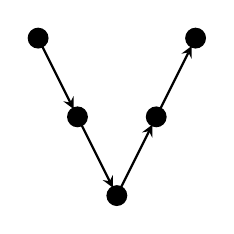
\begin{tikzpicture}[baseline]
	\def \n {2}
	\def \w {0.5}
	\def \r {0.9}
	\def \scale {0.8}
	\begin{scope}
		\foreach \x in {\n,...,1} {
		\node at (-\x*\w,\x) [circle,fill=black,scale=\scale] {};
		\draw [arrow] (-\x*\w,\x) -- (-\x*\w+\r*\w,\x-\r);
		}
		\foreach \x in {1,...,\n} {
		\node at (\x*\w,\x) [circle,fill=black,scale=\scale] {};
		}
			\foreach \x in {1,...,1} {
			\draw [arrow] (\x*\w,\x) -- (\x*\w+\r*\w, \x+\r);
		}
		\node at (0,0) [circle,fill=black,scale=\scale] {};
		\draw [arrow] (0,0) -- (\r*\w, \r);
	\end{scope}
	\end{tikzpicture}}
	\hfill
	\subfloat[][\label{wcycle} W-cycle]{
	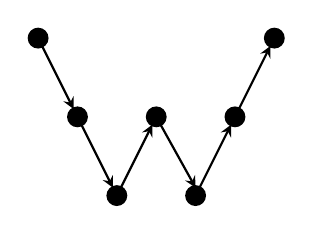
\begin{tikzpicture}[baseline]
	\def \n {2}
	\def \w {0.5}
	\def \r {0.9}
	\def \scale {0.8}
	\begin{scope}
		\foreach \x in {\n,...,1} {
		\node at (-\x*\w,\x) [circle,fill=black,scale=\scale] {};
		\draw [arrow] (-\x*\w,\x) -- (-\x*\w+\r*\w, \x-\r);
		}
		\foreach \x in {0,...,\n} {
		\node at (2*\w + \x*\w,\x) [circle,fill=black,scale=\scale] {};
		}
			\foreach \x in {0,...,1} {
			\draw [arrow] (2*\w + \x*\w,\x) -- (2*\w + \x*\w+\r*\w, \x+\r);
		}
		\node at (0,0) [circle,fill=black,scale=\scale] {};
		\draw [arrow] (0,0) -- (\r*\w, \r);
		\node at (\w,1) [circle,fill=black,scale=\scale]{};
		\draw [arrow] (\w,1) -- (2*\w, 1-\r);
		
	\end{scope}

	\end{tikzpicture}}
	\hfill
	\subfloat[][\label{fmgcycle} F-cycle (full multigrid)]{
	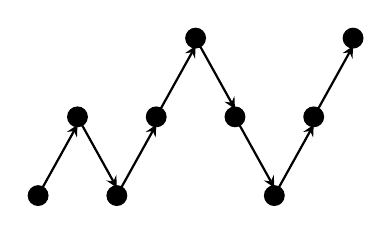
\begin{tikzpicture}[baseline]
	\def \n {3}
	\def \w {0.5}
	\def \r {0.9}
	\def \scale {0.8}
	\begin{scope}
		
		\node at (0,0) [circle,fill=black,scale=\scale] {};
		\node at (\w,1) [circle,fill=black,scale=\scale] {};
		\node at (2*\w,0) [circle,fill=black,scale=\scale] {};
		\node at (3*\w,1) [circle,fill=black,scale=\scale] {};
		\node at (4*\w,2) [circle,fill=black,scale=\scale] {};
		\node at (5*\w,1) [circle,fill=black,scale=\scale] {};
		\node at (6*\w,0) [circle,fill=black,scale=\scale] {};
		\node at (7*\w,1) [circle,fill=black,scale=\scale] {};
		\node at (8*\w,2) [circle,fill=black,scale=\scale] {};
		
		\draw [arrow] (0,0) -- (\w, \r);
		\draw [arrow] (\w,1) -- (2*\w, 1-\r);
		\draw [arrow] (2*\w,0) -- (3*\w, \r);
		\draw [arrow] (3*\w,1) -- (4*\w, 1+\r);
		\draw [arrow] (4*\w, 2) -- (5*\w, 2-\r);
		\draw [arrow] (5*\w, 1) -- (6*\w, 1-\r);
		\draw [arrow] (6*\w, 0) -- (7*\w, \r);
		\draw [arrow] (7*\w, 1) -- (8*\w, 1+\r);
	\end{scope}
	\end{tikzpicture}}
	\caption{\label{fig:mgcycles} Examples of multigrid cycles on a sequence of meshes with three levels.}
\end{figure}







%------------------------------------------------

\section{Components of a multigrid algorithm}

\subsection{Smoothing}

Smoothing is not used to solve the problem, although on its own the smoother may be used as a convergent iterative solver.
Instead, the purpose is to reduce the high frequency errors of the solution on the current grid level.
As mentioned earlier, this is the key idea to multigrid algorithms.
Smoothing is typically done by a SOR method, such as the weighted Jacobi or Gauss-Seidel methods.

\begin{figure}
	% Insert figure of error components for initial iteration phases, want to show low frequency errors are not dampened.
	% Insert figure for how the frequencies decay based on mesh level.
	% Probably use a 1D Helmholtz problem to do this
	\centering
	\includegraphics[draft]{images/placeholder}
	\caption{High frequency errors are damped fast}
\end{figure}


There are two opportunities to perform smoothing operations.
These occur before the restriction to the coarser level (pre-smoothing), then again after the coarse grid correction is applied to the solution on the finer level (post-smoothing).
Different multigrid cycles apply different rules to smoothing, such as when to smooth and how many smoothing iterations to perform.
For example, in the case of a V or W-cycle, both pre-smoothing and post-smoothing are performed.
However, in the case of an S-cycle, no pre-smoothing operations are performed, and only post-smoothing is applied.
For certain problems, this can improve performance because of the reduction of the smoothing operations \cite{iyengar}.


\cite{elman}
The particular choice of smoother in \oomph is between the complex damped Jacobi method and GMRES.
Alternatively, one could choose to implement their own smoother to override the default behaviour.
Generally speaking, 

In this paper, the results and analysis are obtained from using the GMRES solver.




\subsection{Prolongation and restriction}

The procedures for transferring solution data between mesh levels are known as prolongation and restriction.
These operators are built 

Prolongation, otherwise known as interpolation, is the process of transferring data up a level from a coarse grid to a finer grid.
This is done in general by sampling known values to interpolate the unknowns.

Let $\Omega^h$ and $\Omega^{2h}$ be the meshes on the fine and coarse levels, respectively, and let $V^{h}$ and $V^{2h}$ be the finite element spaces on their respective meshes.
Since $\Omega^{h}$ is obtained through refinement of $\Omega^{2h}$, we have that $V^{2h}\subset V^h$.
Then we can define the canonical prolongation operator \cite{volker},
\begin{align}
	I^h_{2h} \, : \, V^{2h} \rightarrow V^h.
\end{align}

As an alternative view of the transfer operator above, we can consider the operator acting on nodal values instead of acting on the members of the finite element space.
Using this approach, if the coarse mesh with a grid resolution $2h$ has $n$ total nodes, and the fine mesh with a grid resolution of $h$ has $m$ total nodes, then
\begin{align}
	I^h_{2h} \, : \, R^m \rightarrow R^n.
\end{align}



Restriction, sometimes known as coarsening or injection, is the `inverse' operation to prolongation.
That is, in the sense that restriction operations perform the opposite action to prolongation.
This process transfers data down a grid level from a fine grid to a coarser grid.

Using the notation as above, we can define the canonical restriction operators \cite{volker},
\begin{align}
	I^{2h}_h \, : \, V^{h} \rightarrow V^{2h}.
\end{align}



On any given mesh level, applying first a restriction then a prolongation, or a prolongation then a restriction, will result in the mesh level remaining constant.
However, it is not necessarily true that the solution data will remain the same.
Since the prolongation operator interpolates data values, certainly there will be some discrepancy in the final result.

Figure \ref{fig:pro_res_ops} is a representation of how the transfer matrices act on points in the mesh.


\begin{figure}[h]
	\centering
	\scalebox{0.4}{
	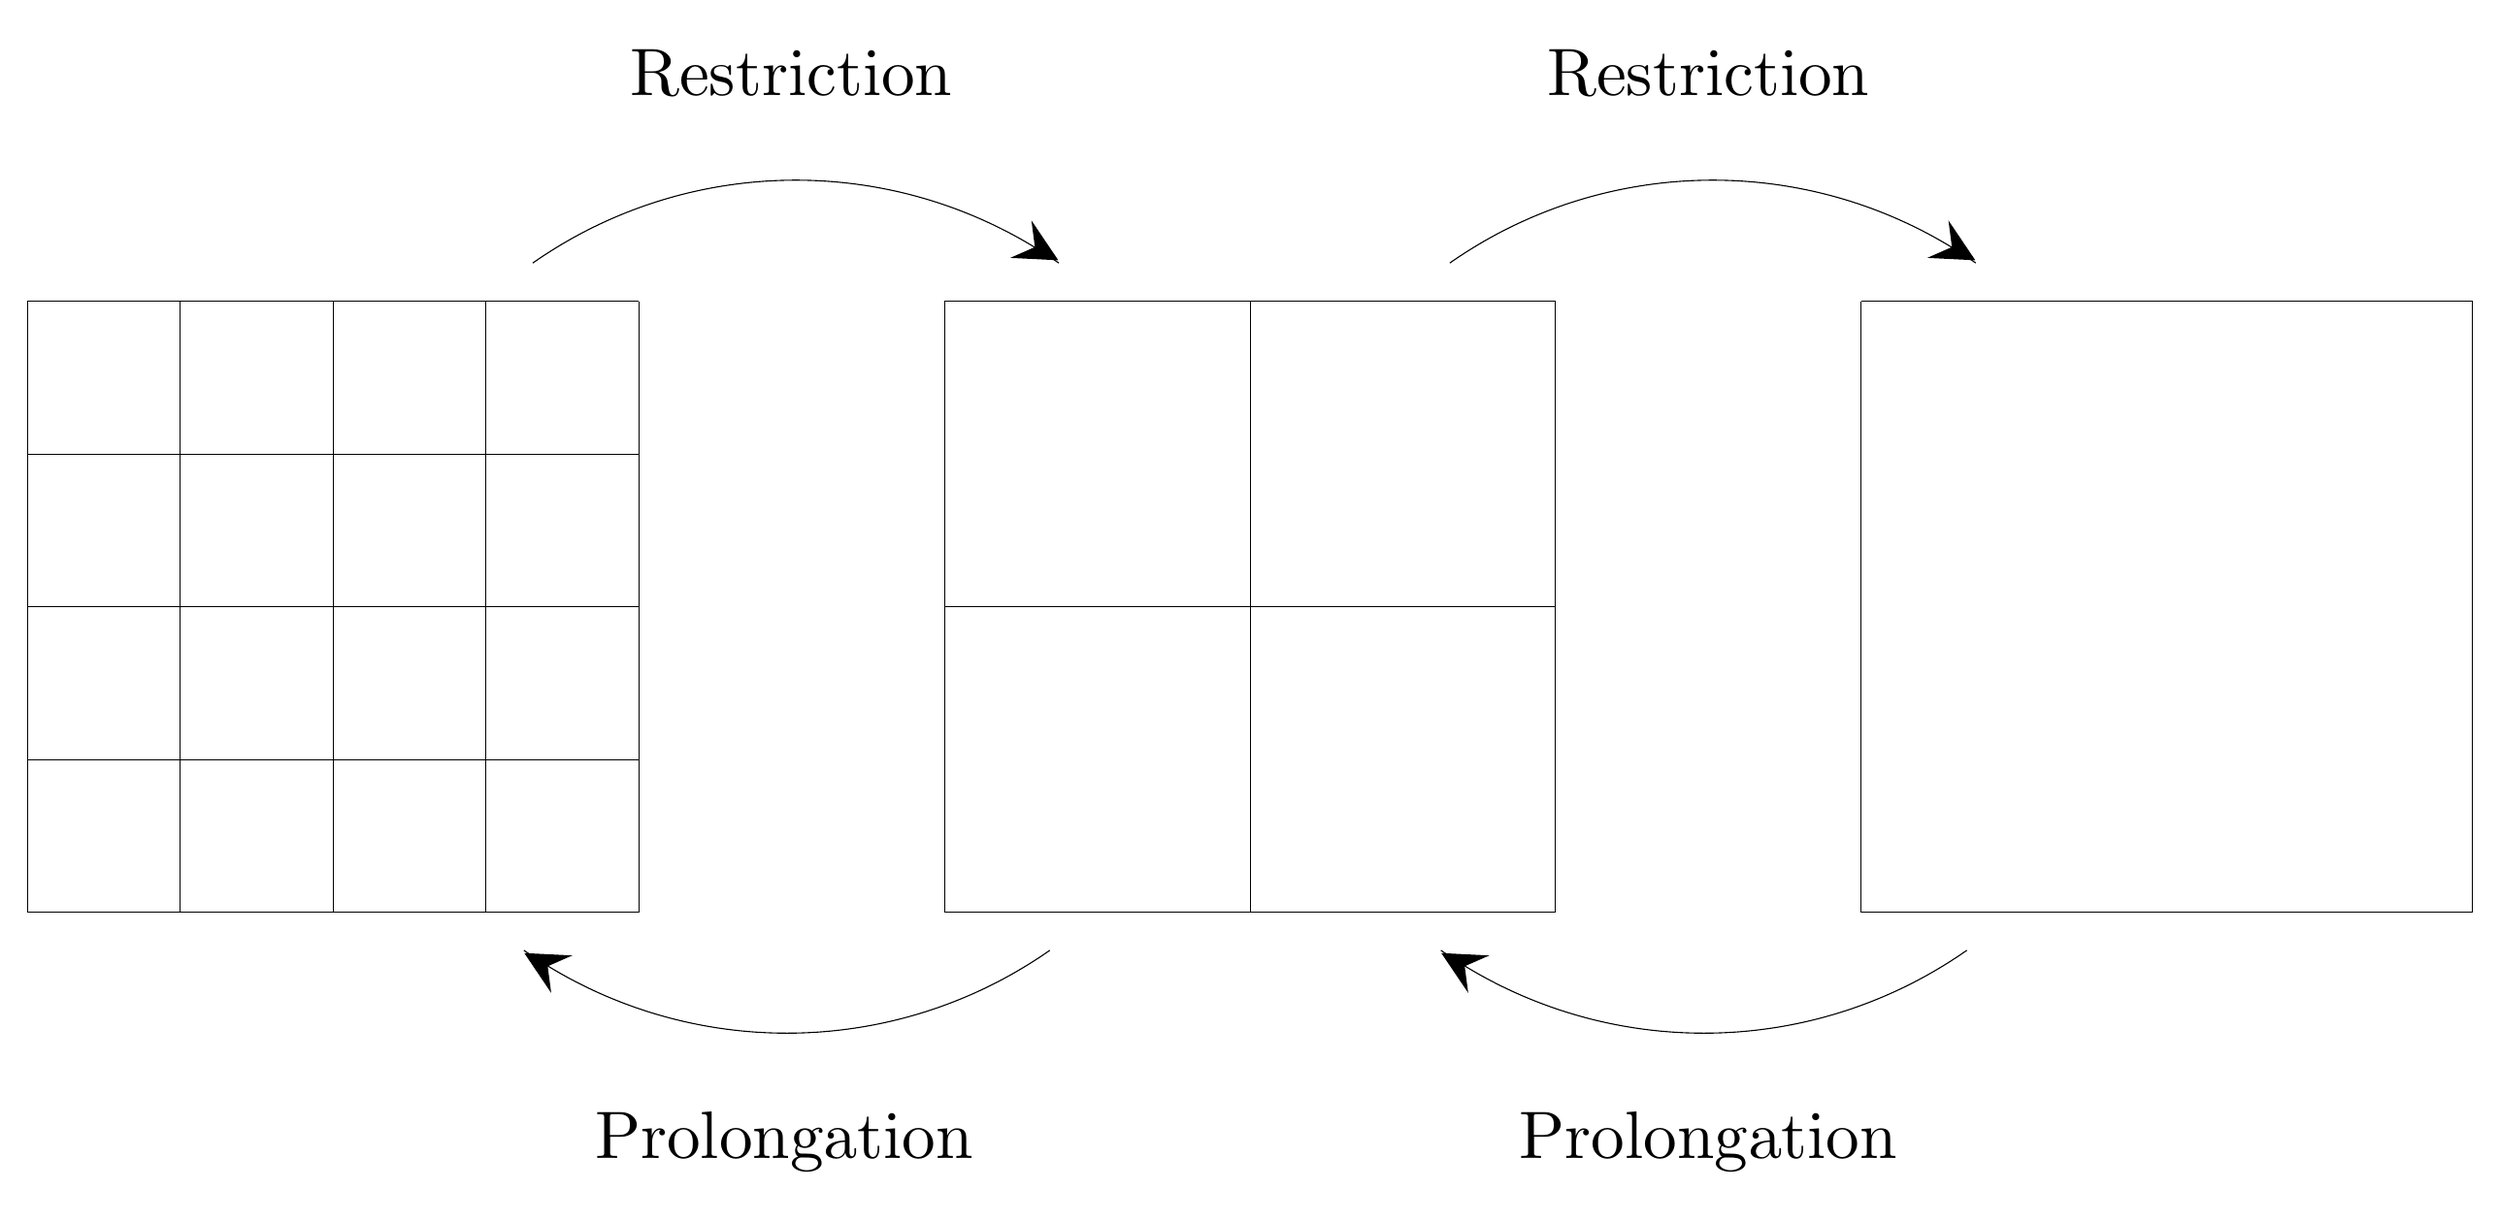
\begin{tikzpicture}[baseline,decoration={markings,mark=at position 0.08 with
		{\arrow[scale=5,>=stealth]{<}}}]
	\centering
	\begin{scope}
	
	% define constants
	\def \w {8}
	\def \d {4}
	\def \textoff {3}
	\def \r {6}
	
	% Draw the grids
	\draw[step=2,black,very thin] (0,0) grid (\w,\w);
	\draw[step=4,black,very thin] (\w+\d,0) grid (2*\w+\d,8);
	\draw[step=8,black,very thin] (2*\w+2*\d,0) grid (3*\w+2*\d,8);
	
	% First text
	\node[anchor=center,scale=2.5] at (\w+\d/2,\w+\textoff) {Restriction};
	\node[anchor=center,scale=2.5] at (\w+\d/2.1,-\textoff) {Prolongation};
	
	% Second text
	\node[anchor=center,scale=2.5] at (2*\w+1.5*\d,\w+\textoff) {Restriction};
	\node[anchor=center,scale=2.5] at (2*\w+1.5*\d,-\textoff) {Prolongation};
	
	% Top arrows
	\draw[postaction={decorate}] (\w+\d+\r/4,\w+0.5) arc (55:125:\r);
	\draw[postaction={decorate}] (2*\w+2*\d+\r/4,\w+0.5) arc (55:125:\r);
	
	% Bottom arrows
	\draw[postaction={decorate}] (\w-\r/4,-0.5) arc (180+55:180+125:\r);
	\draw[postaction={decorate}] (2*\w+\d-\r/4,-0.5) arc (180+55:180+125:\r);
	
	\end{scope}
	\end{tikzpicture}
	}
	
	\caption{\label{fig:pro_res_ops} Prolongation and restriction operators moving between mesh levels.}
\end{figure}



Two transfer operators are required for each mesh level, except for on the finest and coarsest levels.
Instead, a restriction for the coarsest level and a prolongation the matrix is not needed.
All of these are created in the setup phase of the algorithm.
The algorithm used in the \oomph implementation of operator creation process is described below.

To move from a coarse mesh to a fine mesh:
1. Create the fine mesh
2. For each element in the fine mesh
3. For each node in the element
4. Get the local coordinates of the node
5. Interpolate the value of the solution using the coarse mesh solution value and basis functions
6. End loops

Once the prolongation matrix has been created, the restriction matrix is then defined to be the transpose of the prolongation matrix.
Figure \ref{fig:create_prolong_matrix} shows how solution data for a uniform refinement of a single element is performed.

\begin{figure}[h]
	\centering
	\includegraphics[draft]{images/placeholder}
	\caption{Prolongation matrix creation process. \label{fig:create_prolong_matrix}}
\end{figure}




\subsection{Grid hierarchy}

We will restrict our discussion to uniform structured grids in order to focus on the details of multigrid.
Mathematically, we require only the grid hierarchy so the specific internals of the individual grids is a technical detail that we will omit. 

% We want to discuss how the grid hierarchy is computed and used within oomph-lib.
The grid hierarchy used by multigrid in \oomph is generated by... 



\begin{figure}[h]
	% Show initial refinement, want to show how the hierarchy is created within oomph-lib
	\centering
	\includegraphics[draft]{images/placeholder}
	\caption{Example of a grid hierarchy created for multigrid in \oomph.}
\end{figure}





%------------------------------------------------

\section{Multigrid as a preconditioner}
\label{sec:precond}

\subsection{Block preconditioning}

% Talk about block preconditioning in regards to complex Helmholtz problem
% The block structure, derivation...
% Enumeration of the unknowns and equations. Real part first, imaginary part second

As mentioned in chapter \ref{sec:problem}, the Helmholtz equation we are interested in is complex-valued.
Since \oomph does not natively handle complex arithmetic, complex numbers are instead stored as 2D vectors.
The first component of the vector is the real part of the complex number, and the second component is the imaginary part.

For a specific enumeration of the unknowns, we obtain a matrix whose structure allows us to solve the problem more efficiently.
In our case, we first compute the contribution for all of the real unknowns, then the contribution for the imaginary unknowns.
This gives rise to a Jacobian matrix with block structure
\begin{align}
	A = \begin{pmatrix}
		A_r & -A_c \\ A_c & A_r
	\end{pmatrix}.
\end{align}
Here, $A_r$ is the real part of the discretisation and $A_c$ is the imaginary part.

Given this matrix with a block structure, we will want to use a block preconditioner as our preconditioning matrix.




\subsection{Multigrid preconditioning}

As an alternative to using multigrid as an iterative solver, it is possible to instead perform multigrid iterations to partially solve the linear system, then perform a solve with an additional linear solver on the preconditioned system.
This gives an effective method  

On its own, the linear solver is not as effective as the preconditioned linear solver.


We reduce the tolerance of the mg solver and 





\subsection{FGMRES}

Multigrid preconditioning leads to a variable preconditioner.
That is, between iterations, the preconditioning matrix changes.

Because of this, the standard GMRES method is not a suitable choice of smoother.
Instead, the flexible version of the GMRES algorithm, appropriately named FGMRES, may be used instead.

Only capable of preconditioning on the right


This method was proposed by Saad in \cite{fgmres}.
For a more detailed description of the FGMRES algorithm, readers are directed to this paper.



\chapter{Results}

\def\figwidth{0.7\columnwidth}


What results did we gather?
What machine did we use?

Need a general discussion for each



\begin{figure}
    \centering
    
    \pgfplotstableread{
    1 2.03073e-06
    0.5 2.54252e-07
    0.25 3.17945e-08
    0.125 3.97473e-09
    0.0625 4.96869e-10
    }\datatable

    \begin{tikzpicture}
        \centering
    \begin{loglogaxis}[
    xlabel={$h$},
    ylabel={Error},
    xmin=0.01, xmax=1.1,
    grid=major,
    width=\figwidth
    % /pgfplots/log ticks with fixed point,
    ]
    
    \addplot [only marks,fill=black] table {\datatable};

    \addplot table[y={create col/linear regression={y=1}}] {\datatable} 
    coordinate [pos=0.8] (A)
    coordinate [pos=0.3] (B);

    \xdef\slope{\pgfplotstableregressiona} % save the slope parameter
    \draw (B) -| (A)  % draw the opposite and adjacent sides of the triangle
    node [pos=0.25, anchor=south] {1} % label the horizontal line
    node [pos=0.75,anchor=east] {\pgfmathprintnumber{\slope}} %label the vertical line
    ;

    % \addlegendentry{$\pgfmathprintnumber{\pgfplotstableregressiona}$}

    \end{loglogaxis}
    \end{tikzpicture}
    \caption{This is a figure.}
\end{figure}


\begin{figure}
    \centering
    
    \pgfplotstableread{
    1 2.03073e-06
    0.5 2.54252e-07
    0.25 3.17945e-08
    0.125 3.97473e-09
    0.0625 4.96869e-10
    }\datatable

    \begin{tikzpicture}
        \centering
    \begin{loglogaxis}[
    xlabel={$h$},
    ylabel={Error},
    xmin=0.01, xmax=1.1,
    grid=major,
    width=\figwidth
    % /pgfplots/log ticks with fixed point,
    ]
    
    \addplot [only marks,fill=black] table {\datatable};

    \addplot table[y={create col/linear regression={y=1}}] {\datatable} 
    coordinate [pos=0.8] (A)
    coordinate [pos=0.3] (B);

    \xdef\slope{\pgfplotstableregressiona} % save the slope parameter
    \draw (B) -| (A)  % draw the opposite and adjacent sides of the triangle
    node [pos=0.25, anchor=south] {1} % label the horizontal line
    node [pos=0.75,anchor=east] {\pgfmathprintnumber{\slope}} %label the vertical line
    ;

    % \addlegendentry{$\pgfmathprintnumber{\pgfplotstableregressiona}$}

    \end{loglogaxis}
    \end{tikzpicture}
    \caption{This is a figure.}
\end{figure}
\chapter{Conclusion}

The work completed in this project has led to the successful development of a solver for the Helmholtz equation in Fourier decomposed cylindrical coordinates.
We have built on the existing machinery for the Helmholtz equation in Cartesian coordinates and created the necessary extensions required for finding the solution in this case.

Results gathered in the previous chapter demonstrate that the cylindrical and Cartesian Helmholtz equations behave similarly.
When $k^2$ becomes larger, this is less so, however the method is still convergent for large values of the wavenumber.

A discussion of the issues that might have caused problems were detailed.
For example, the problem with variable coefficients for the multigrid iteration and the indefiniteness of the Helmholtz discretisation.
In the end, these issues were succesfully overcome or did not pose a problem at all.
The shifted-Laplacian preconditioner works well in the change of variables, with results consistent with the existing literature.

In summary, it has been shown that a multigrid based preconditioner for FGMRES is a viable method for solving the finite element discretisation of the Fourier decomposed Helmholtz equation in cylindrical coordinates.





% -------------------------------------

\section{Further work}

This work has only considered and implementated Dirichlet boundaries.
A first step to extend the results would be to introduce other boundary conditions, including absorbing boundary conditions.
The simplifications were appropriate for initial work, but applications likely will involve non-essential boundaries.
For this work to be of any use in the future, this should be handled first.

Increasing the Fourier wavenumber $N$ causes issues for both the multigrid and SuperLU solvers.
This is likely caused because the equation is incorrectly scaled.
Appropriately scaling the equation should resolve the problem.
Alternatively, we can shift the mesh to increase the minimum value of $r$ so that it is approximately equal to $N$.
Implementing a more robust method for handling large $N$ and an accompanying convergence study should be performed.



\bibliography{bibliography}
\bibliographystyle{plain}

\ifdefined\nopreamble
\else
  \appendix
  \chapter{Code listings}

  This code has been adapted from existing sources within the \oomph codebase.
  For a complete directory of code, consult the \oomph repository at the website \cite{oomph}.
  The changes included here are those necessary for this project.

  \section{Driver code}
  \lstinputlisting[language=C++,caption=Filename: main.cc. Driver code containing main entry point to the program.]{../oomph/user_drivers/billy/main.cc}

  \clearpage
  \section{Element code}
  \lstinputlisting[language=C++,caption=Filename: refineable\_pml\_helmholtz\_elements.cc. Element code for the refineable version of the Fourier decomposed Helmholtz equation.]{../oomph/user_drivers/billy/SourceFiles/refineable_pml_helmholtz_elements.cc}
\fi
\end{document}
